%% LyX 2.0.6 created this file.  For more info, see http://www.lyx.org/.
%% Do not edit unless you really know what you are doing.
\documentclass{article}
\usepackage{mathpazo}
\renewcommand{\ttdefault}{mathpazo}
\usepackage[T1]{fontenc}
\usepackage[latin9]{inputenc}
\usepackage{geometry}
\geometry{verbose,columnsep=20pt}
\usepackage{fancyhdr}
\pagestyle{fancy}
\usepackage{float}
\usepackage{booktabs}
\usepackage[unicode=true,pdfusetitle,
 bookmarks=true,bookmarksnumbered=false,bookmarksopen=false,
 breaklinks=false,pdfborder={0 0 1},colorlinks=false]
 {hyperref}
\usepackage{breakurl}

\makeatletter

%%%%%%%%%%%%%%%%%%%%%%%%%%%%%% LyX specific LaTeX commands.
%% Because html converters don't know tabularnewline
\providecommand{\tabularnewline}{\\}

\@ifundefined{date}{}{\date{}}
%%%%%%%%%%%%%%%%%%%%%%%%%%%%%% User specified LaTeX commands.
%%%%%%%%%%%%%%%%%%%%%%%%%%%%%%%%%%%%%%%%%
% Journal Article
% LaTeX Template
% Version 1.3 (9/9/13)
%
% This template has been downloaded from:
% http://www.LaTeXTemplates.com
%
% Original author:
% Frits Wenneker (http://www.howtotex.com)
%
% License:
% CC BY-NC-SA 3.0 (http://creativecommons.org/licenses/by-nc-sa/3.0/)
%
%%%%%%%%%%%%%%%%%%%%%%%%%%%%%%%%%%%%%%%%%

%----------------------------------------------------------------------------------------
%	PACKAGES AND OTHER DOCUMENT CONFIGURATIONS
%----------------------------------------------------------------------------------------
\clubpenalty10000
\widowpenalty10000
\displaywidowpenalty=10000

\usepackage[numbers]{natbib}
\usepackage{tikz}

\usepackage{tabularx}
\usepackage{arydshln}

\usepackage{footmisc}


%\newcommand*{\textlabel}[2]{%
%  \edef\@currentlabel{#1}% Set target label
%  \phantomsection% Correct hyper reference link
%  #1\label{#2}% Print and store label
%}

\usepackage{lipsum}% Package to generate dummy text throughout this template

% Use the Palatino font
% Use 8-bit encoding that has 256 glyphs
\linespread{1.05} % Line spacing - Palatino needs more space between lines
\usepackage{microtype}% Slightly tweak font spacing for aesthetics

%\usepackage[author-year]{natbib}   

% Document margins
\usepackage{multicol}% Used for the two-column layout of the document
\usepackage[hang, small,labelfont=bf,up,textfont=it,up]{caption}% Custom captions under/above floats in tables or figures
% Horizontal rules in tables
% Required for tables and figures in the multi-column environment - they need to be placed in specific locations with the [H] (e.g. \begin{table}[H])
% For hyperlinks in the PDF

\usepackage{lettrine}% The lettrine is the first enlarged letter at the beginning of the text
\usepackage{paralist}% Used for the compactitem environment which makes bullet points with less space between them

\usepackage{abstract}% Allows abstract customization
\renewcommand{\abstractnamefont}{\normalfont\bfseries} % Set the "Abstract" text to bold
\renewcommand{\abstracttextfont}{\normalfont\small\itshape} % Set the abstract itself to small italic text

\usepackage{titlesec}% Allows customization of titles
\renewcommand{\thesection}{\Roman{section}} % Roman numerals for the sections
\renewcommand{\thesubsection}{\Roman{subsection}} % Roman numerals for subsections
\titleformat{\section}[block]{\large\scshape\centering}{\thesection.}{1em}{} % Change the look of the section titles
\titleformat{\subsection}[block]{\large}{\thesubsection.}{1em}{} % Change the look of the section titles

\usepackage{fancyhdr}% Headers and footers
 % All pages have headers and footers
\fancyhead{} % Blank out the default header
%\fancyfoot{} % Blank out the default footer
\fancyhead[C]{Recent Advances in Multicore Systems  $\bullet$ SoSe 2014, TU Berlin} % Custom header text
%\fancyfoot{\thepage} % Custom footer text

%----------------------------------------------------------------------------------------
%	TITLE SECTION
%----------------------------------------------------------------------------------------

\title{\vspace{-10mm}\fontsize{24pt}{10pt}\selectfont\textbf{Parallelization of Video Encoding on CPU+GPU}} % Article title

\author{
\large
\textsc{Mirko Liebender}\\[2mm] % Your name
\normalsize Technische Universit�t Berlin \\ % Your institution
\normalsize {mirko@mailbox.tu-berlin.de} % Your email address
\vspace{-5mm}
}


%----------------------------------------------------------------------------------------


\definecolor{rosso}{RGB}{220,57,18}
\definecolor{giallo}{RGB}{255,153,0}
\definecolor{blu}{RGB}{102,140,217}
\definecolor{verde}{RGB}{16,150,24}
\definecolor{viola}{RGB}{153,0,153}

\makeatletter

\tikzstyle{chart}=[
    legend label/.style={font={\scriptsize},anchor=west,align=left},
    legend box/.style={rectangle, draw, minimum size=5pt},
    axis/.style={black,semithick,->},
    axis label/.style={anchor=east,font={\tiny}},
]

\tikzstyle{bar chart}=[
    chart,
    bar width/.code={
        \pgfmathparse{##1/2}
        \global\let\bar@w\pgfmathresult
    },
    bar/.style={very thick, draw=white},
    bar label/.style={font={\bf\small},anchor=north},
    bar value/.style={font={\footnotesize}},
    bar width=.75,
]

\tikzstyle{pie chart}=[
    chart,
    slice/.style={line cap=round, line join=round, very thick,draw=white},
    pie title/.style={font={\bf}},
    slice type/.style 2 args={
        ##1/.style={fill=##2},
        values of ##1/.style={}
    }
]

\pgfdeclarelayer{background}
\pgfdeclarelayer{foreground}
\pgfsetlayers{background,main,foreground}


\newcommand{\pie}[3][]{
    \begin{scope}[#1]
    \pgfmathsetmacro{\curA}{90}
    \pgfmathsetmacro{\r}{1}
    \def\c{(0,0)}
    \node[pie title] at (90:1.3) {#2};
    \foreach \v/\s in{#3}{
        \pgfmathsetmacro{\deltaA}{\v/100*360}
        \pgfmathsetmacro{\nextA}{\curA + \deltaA}
        \pgfmathsetmacro{\midA}{(\curA+\nextA)/2}

        \path[slice,\s] \c
            -- +(\curA:\r)
            arc (\curA:\nextA:\r)
            -- cycle;
        \pgfmathsetmacro{\d}{max((\deltaA * -(.5/50) + 1) , .5)}

        \begin{pgfonlayer}{foreground}
        \path \c -- node[pos=\d,pie values,values of \s]{$\v\%$} +(\midA:\r);
        \end{pgfonlayer}

        \global\let\curA\nextA
    }
    \end{scope}
}

\newcommand{\legend}[2][]{
    \begin{scope}[#1]
    \path
        \foreach \n/\s in {#2}
            {
                  ++(0,-10pt) node[\s,legend box] {} +(5pt,0) node[legend label] {\n}
            }
    ;
    \end{scope}
}


%------------------------------------------------------------------------------
\makeatother

\begin{document}


\maketitle % Insert title


\thispagestyle{fancy} % All pages have headers and footers

\reversemarginpar
%----------------------------------------------------------------------------------------
%	ABSTRACT
%----------------------------------------------------------------------------------------

\begin{abstract}
Video en- and decoding is nowadays a central technology on many platforms and systems in all over the world. It is used in computers, TVs, smartphones, streaming platforms, video conferences, blu-rays etc.
It has been developed over the past decades and therefore many different video codecs and algorithms were developed over time to solve certain purposes (e.g., H.265/HEVC, H.264/AVC, MPEG-2) and to address requirements of many applications.\\
Since the demand of high resolution videos is more and more increasing these codecs aim to reach a high compression rate while maintaining a good quality. The cost of this approach is always a higher computing requirement 
(e.g. HEVC aims to reach half the size while maintaining the same quality as AVC \todo{this example does not show the higher computation requirement for HEVC, remove it}).\\
In order to meet these requirements many different basic approaches are researched. This articles mainly \todo{typo focusses} on the graphic processing units (GPU) and the encoding process.\\
GPUs have emerged as a coprocessing unit for central processing units (CPUs) to accelerate certain logical parts of the encoding process.\\
GPUs consist of a large amount of streaming processors, which allow them to execute a lot of operations in parallel. Because GPUs consist of a \todo{capitalize Single Instruction Multiple Data} (SIMD) architecture  and the fact that data synchronisation between CPU and GPU is considered a bottleneck, it is a rather complex task to efficiently use this immense parallel performance while handling all the constraints of the GPUs .\\
In this paper three different strategies to address this challenge are reviewed. Two of them propose parallel strategies for the H.264 codec and one for the H.265 codec. They all reach certain speed ups in their field but are not necessarily developed for wide use.
\end{abstract}
%----------------------------------------------------------------------------------------
%	ARTICLE CONTENTS
%----------------------------------------------------------------------------------------


\begin{multicols}{2} % Two-column layout throughout the main article text



\section{Introduction}
\label{sec:intro}
The increasing demand of high quality video communication in nearly every part of the electronic entertainment area and the tremendous growth of video contents on the Internet pushed the development of high efficient compression methods. These codecs however are always limited by the average power of the computers used at there design time. \\
Especially with High Definition (HD) video content going to be replaced by beyond-HD content, like Ultra High Definition (UHD), a high compression rate is very important due to the limitations in transfer rate in many areas.\\
The H.264/AVC \cite{H264_Overview} codec was designed to reach a significant improvement regarding the distortion efficiency compared to existing standards. Efforts have been enhanced compression rate and a network-friendly representation for conversational and non-conversational applications. It also aimed to be flexible to be used on many different system types.\\
At the time, May 2003, parallelism of the algorithm H.264 itself wasn't really taken into consideration. Due to the fact that a standard personal computer around 2003 didn't have a multi core processor, parallelism wasn't considered important enough. The utilization of GPUs was also mostly limited to video gaming. Frameworks like CUDA \footnote{Compute Unified Device Architecture} or OpenCL\footnote{Open Computing Language} were just developed recently.\\
The H.265/HEVC \cite{H265_Overview} standard is the most recent project\footnote{released 2013} of the ITU-T Video Coding Experts Group (VCEG) and the ISO/IEC Moving
Picture Experts Group (MPEG) standardization organizations. The codec aims to reach half the size of the existing standards while maintaining the same quality, therefore significantly improve the compression rate. This goal is mainly reached by optimizing the use of parallel processing architectures.\\
Both codecs are very similar and inherited the known hybrid Motion Estimation (ME)/Motion Compensation (MC) followed by transform and entropy coding framework adopted by H.261 \cite{H261_Overview} since 1994.\\

For H.264/AVC being available since 2003, a lot of work has been contributed to optimize parallelism for the algorithm. The Motion Estimation (ME) is one of the most compute intensive parts of both H.264 and H.265. A lot of studies have been made over the last years to research propose strategies to utilize GPUs to undertake ME. \\
In \cite{ME1} a multi-pass method is proposed to unroll and rearrange the nested loops of ME and implement it on the GPU. They reached a speed-up of 2 to 14 times respectively for integer-pel ME and half-pel ME.\\

The authors of \cite{ME2} performed ME on a block-by-block basis on the GPU to overcome the dependency problem between blocks, which is often ignored by algorithms. The study group compared their GPU algorithm with a self optimized Single Instruction Multiple Data (SIMD) algorithm for CPU. They reached a speed-up of up to 10 times, but it has to be taken into account, that their algorithm has to be optimized for each GPU differently.\\

The article \cite{ME3} proposed an adoption of a parallel small diamond search on the GPU to speed-up the ME. They were greatly limited by the memory bandwidth but reached a small speed-up around 10\% but with a small loss in quality.\\

In \cite{ME4} they developed a scalable ME algorithm for GPUs that focusses on the computation power and takes re-usability of data into account. The scalability regarding different number of cores for  GPUs of the same architecture was also an important goal for the study to be used in the future. They reached speed-ups up to 3 times for their optimized algorithm on GPU.\\

Another approach, \cite{deblock1}, considered the possibility to parallelize the deblocking filter on GPU. Usually deblocking is done on the CPU in serial due to its data dependencies. The articles approach tries to reduce these dependencies to make use of the parallel computation power of GPUs. For their implemented deblocking filter they reached speed-ups around 10 to 20 times compared to a state-of-the-art CPU deblocking filter.\\

In this paper three approaches are reviewed, which try to exploit the possible parallel performance of modern GPUs for the modern video codecs H.264 and H.265. \\
In section \ref{sec:background} a short overview on the two video coding techniques is given. In the following section \ref{sec:paper} the three papers \cite{Paper1}, \cite{Paper2} and \cite{Paper3} and their proposals are presented in detail. After that the experimental results of the papers are presented and compared in section \ref{sec:results}.\\
In the last section \ref{sec:conclusion} a conclusion is given.

\section{Background}
\label{sec:background}
In the past decade new video coding standards have achieved state-of-the-art coding performance. H.264/AVC typically requires 60\% or less of the bit rate compared to previous \todo{typo standars} to achieve the same reconstruction quality \cite{H264_Overview}. In comparison, H.265/HEVC requires around 50\% less then H.264/AVC. Next, a short overview on both codecs is given.\\
\\
The H.264/AVC \cite{h264joint}, \cite{H264_Overview} video coding algorithm is depicted in block diagram \ref{h264}.

\begin{figure}[H]
\centerline{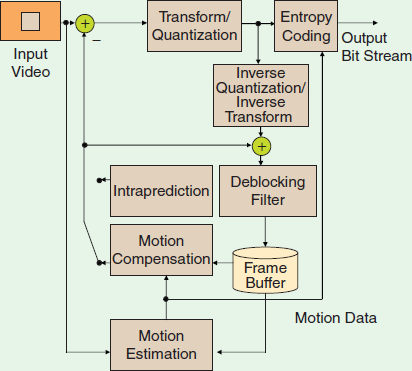
\includegraphics[scale=0.5]{pics/H264_Blockschaltbild}} % The bounding box is set manually in this example. Useful for some .pdf figures.
\caption{\label{h264}{\it H.264/AVC encoding algorithm (taken from \cite{Paper1})}}
\end{figure} % [width=5in,bb= 36 253 574 500]

It is designed on a block-based hybrid approach which has been a wide spread used approach for many video codecs. \todo{an explanation for h264 figure is expected} On the one hand it exploits spatial correlation between neighbouring pixels and on the other hand it uses the correlation between neighbouring pictures. This method has been used by many codecs before, but there are many highlights compared to previous standards like MPEG-2 \cite{MPEG2}, from which some are shown next.\\
Variable block-size motion compensation (VBSMC) is supported with different block sizes downto 4x4 for luma motion compensation blocks. H.264 also allows quarter-sample-accurate motion compensation. Most standards previous to H.264 only featured half-sample-accuracy.\\ The decoupling of referencing order from display order of images ensures that the flexibility of the encoder is only constraint to the memory. It is also possible to use all encoded pictures for further referencing, which isn't the case in other previous codecs.\\
Another important highlight is the in-loop deblocking filter, which filters the blocking artifacts that occur at block-based video coding algorithms. This filter is combined with the motion-compensation prediction loop to use the improvement in quality from the deblocking filter for better inter-prediction.\\
An additional feature from the H.263 codec was the entropy coding which is a standard feature in H.264. The CABAC (context-adaptive binary arithmetic coding) \cite{cabac} is a powerful entropy coding algorithm to gain further compression without loosing quality at all.\\
There are many more highlights of the H.264 codec that can't all be named in this article due to its size, but that can be found in \cite{H264_Overview}.\\
\\


The H.265/HEVC \cite{H265_Overview} block diagram is depicted in \ref{h265}. 


\begin{figure*}[ht]
\centerline{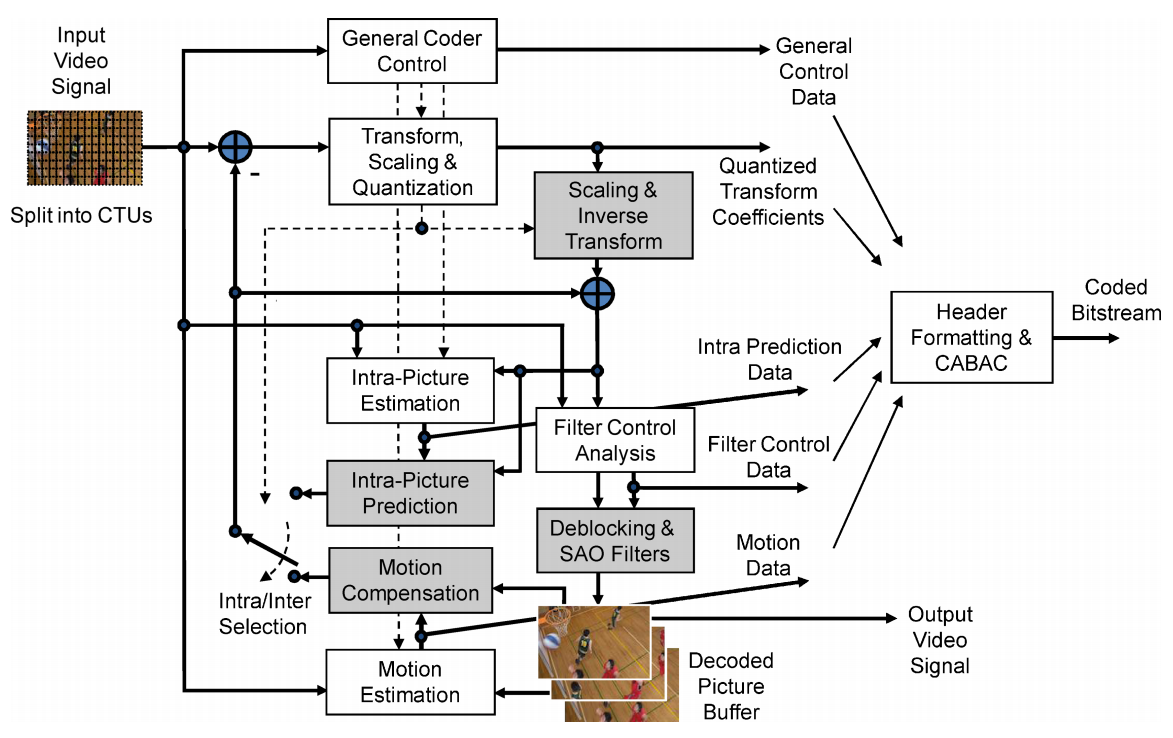
\includegraphics[scale=0.45]{pics/H265_Blockschaltbild}} % The bounding box is set manually in this example. Useful for some .pdf figures.
\caption{\label{h265}{\it H.265/HEVC encoding algorithm (taken from \cite{H265_Overview})}}
\end{figure*} % [width=5in,bb= 36 253 574 500]

The codec is very similar to H.264 but has some major improvements regarding parallelization and aims to reach the goal of having around half the size of an H.264 video while maintaining the same quality. Some of the many highlights are mentioned below.\\
\\
In H.265 a new structure for handling the macroblocks was introduced, the coding tree units (CTU). They basically replace the macroblocks from the H.264 codec. They are variable in size with a maximum of 64x64, for it is larger than the maximum macroblock size. They consist of luma coding tree blocks (CTB) and the corresponding chroma CTBs and can be partitioned into smaller blocks, called coding blocks (CB). 3 CBs form one coding unit (CU). This CTU/CTB structure allows the H.265 to be more flexible for inter and intra prediction of the blocks.\\
The H.265 codec also supports variable prediction block sizes from 64x64 down to 4x4 samples.\\
\todo{The deblocking filter and the entropy coder are still the same like in H.264, but with some improvements towards throughput speed and parallelism. deblocking filter is not the same in H.264 and H.265, say something like the deblocking filter is simplified for parallel processing compared to H.264}.
Additionally to the deblocking filter a sample adaptive offset filter was added, which allows the image to be better reconstructed by applying another advanced filter after the deblocking filter. 
\todo{This filter improves the result significantly by just using a few percent more computation time, change to, SAO was proposed to reduced the distortion between the reconstructed pixels and the original pixels. 
bit rate improvements ranging from 1.3\% to 3.0\% are observed, see paper ``Sample Adaptive Offset for HEVC'', and better add it as a reference}.


\section{Parallel video encoding}
\label{sec:paper}
\subsection*{GPU based Fast Motion Estimation}
\label{sec:paper1}
In \cite{Paper1} the authors designed and developed a GPU-based fast Motion Estimation (ME) algorithm and implemented it based on the H.264 JM 14.2 reference software. 
Their goal was to harness the GPU parallel capabilities by breaking off dependencies with tiling frames and than examine how to trade-off the speed-up with Rate Distortion (RD) performance.\\
For that purpose they implemented Motion Estimation on the GPU based on \textit{simplified unsymmetrical multihexagon search \\(smpUMHexagonS)} \cite{yi2005improved}, 
which is one of the fast ME algorithms adopted by the H.264 JM reference software. 
They selected smpUMHexagonS because it can archieve very good tradeoff between computational complexity and coding efficiency. 
It is not only reported to achieve up to 94\% reduction in execution time in ME on a Pentium 4 with comparable RD efficiency, 
when compared with the fast full search in the JM software \cite{yi2005improved}, but also to be very compact and 
therefore meeting the memory constraint of the GPU. Although full search is usually not used in encoding, due its inefficiency, 
the comparison shows, that the compact size of the algorithm is rather important to execute it on the GPU.\\
%
\\
The main problem of ME on the GPUs is the dependency between the different blocks. To find MVs the smpUMHexagonS algorithm is always calculating the minimal Langrangian cost $D + \lambda R$, where D is the sum of
absolute differences (SAD) between the current block and the candidate, and R is the bitrate
to encode the MV dependencies between neighbouring blocks. This implicates a certain dependency between neighbouring blocks. This however is the main reason, why parallelization of ME is very difficult to realise.
The authors of this paper took an easy approach to avoid this problem by just ignoring some dependencies. 
By doing so they set every MV on a tiles boarder to zero and therefore are not always able to calculate the best MVs, resulting in a loss of quality. Another drawback is, 
that the motion vector prediction of the algorithm can't fully be utilized due to the fact, that MVs of neighbouring tiles are unknown. 
It seems that the authors focused their algorithm optimization on the possible speed-up of tiling regardless the quality of the encoded video.\\
\\
The tiling of a frame is presented in figure \ref{tiling}. Each tile consists of \textit{K x L} macroblocks and is to be processed by a single GPU thread concurrent with the other tiles. 
the number of tiles per frame is therefore dependent on the variables \textit{K} and \textit{L}, which describe the width and the hight of each tile.

\begin{figure}[H]
\centerline{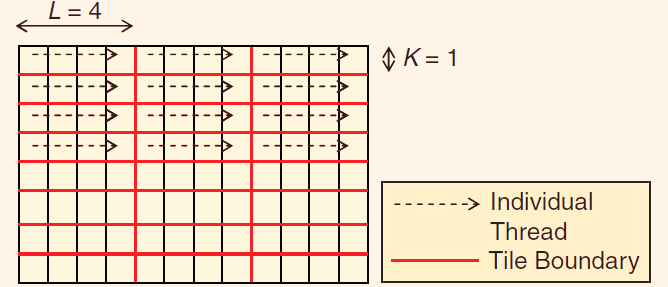
\includegraphics[scale=0.35]{pics/tiling}} % The bounding box is set manually in this example. Useful for some .pdf figures.
\caption{\label{tiling}{\it GPU-based fast ME: the current frame is divided into
multiple tiles to facilitate parallel processing in ME. Here each square represents an MB. (taken from \cite{Paper1})}}
\end{figure}


\subsection*{Dynamic model for parallel H.264/AVC video encoding
on hybrid GPU+CPU}
\label{sec:paper2}
In \cite{Paper2} they proposed a dynamic model for parallel H.264/AVC video encoding on hybrid GPU+CPU. 
First they analysed the dependencies of the encoding process of H.264/AVC. 
For their model to work they needed concrete information on every part of the algorithm itself and its possibility to be parallelised. 
These dependencies analysis showed, that parallel processing can only be considered within the scope of a single frame. 
Inter-prediction usually can not start before updating the list of referenced frames. 
The deblocking-filter for instance can not be applied on two different regions of each slice, because it has intra-frame dependencies, one point that was improved in H.265. \\
The conclusion of the analyses however indicates, that the best possibilities to process H.264 in parallel are the interpolation and the ME. 
Motion estimation is like already mentioned the most compute intense part of the algorithm anyway and also the main approach of the other papers reviewed in this article. 
\todo{Interpolation however is also interesting, because GPUs are mostly equipped with an interpolation unit, 
Here the interpolation unit is a hardware solution, however, we are talking about software solution based on GPU, therefore delete this sentence to avoid confusion}.\\

\begin{figure}[H]

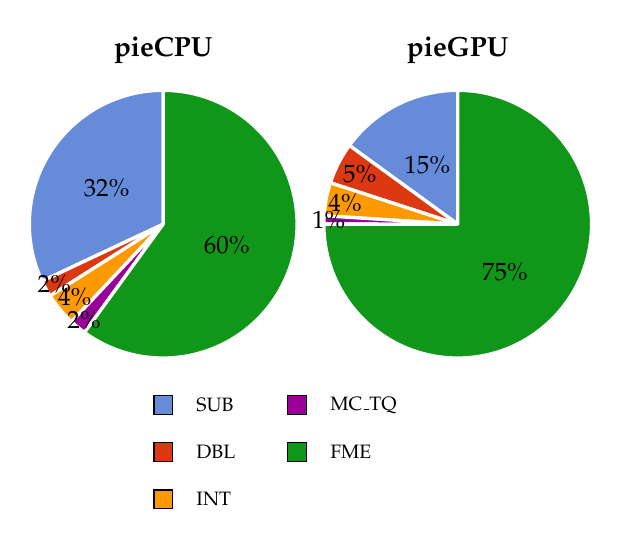
\begin{tikzpicture}
[
    pie chart,
    slice type={sub}{blu},
    slice type={dbl}{rosso},
    slice type={int}{giallo},
    slice type={mctq}{viola},
    slice type={fme}{verde},
    pie values/.style={font={\small}},
    scale=1.7
]
	\pie{\hypertarget{pie}{CPU}}{32/sub,2/dbl,4/int,2/mctq,60/fme}
	\pie[shift={(2.2cm,0cm)}]{\hypertarget{pie}{GPU}}{15/sub,5/dbl,4/int,1/mctq,75/fme}

    \legend[shift={(0 cm,-1 cm)}]{{SUB}/sub, {DBL}/dbl, {INT}/int}
	\legend[shift={(1 cm,-1 cm)}]{{MC\_TQ}/mctq, {FME}/fme}

\end{tikzpicture}
\caption{\label{dynamic_cpu_gpu}{\it Breakdown of the H.264/AVC interprediction-loop processing time measured by \cite{Paper2}; (FME: full-
pixel ME; SUB: sub-pixel ME; INT: interpolation; DBL: deblocking filter; MC TQ: di-
rect transform, quantization, dequantization and inverse transform) (data taken from \cite{Paper2})}}
\end{figure}

Figure \ref{dynamic_cpu_gpu} represents a breakdown of the H.264/AVC processing time for both CPU and GPU implementations, regarding the several encoding modules. These results were obtained by measuring  a highly optimized implementation on an Intel Core i7 CPU and on an NVIDIA GeForce GTX 580 GPU. However, the author doesn't really say which algorithm was used and what optimizations were done. But for the study the breakdown was used to determine the importance of each part of the codec algorithm. It can clearly be seen, that ME is the dominant module with 60\% on the CPU and 75\% on the GPU.

Because the heterogeneous structure of the H.264/AVC encoder includes modules with very different characteristics regarding the data dependencies and parallelization potential the authors analysed the possibility of minimizing the encoding time by efficiently distributing the several tasks on the CPU and on the GPU.\\

They created an algorithm which evaluates the performance of the GPU and CPU for certain parts of the encoding algorithm at runtime. That means that they chose a dynamic approach to evaluate the performance and change the amount of work for each device for each step of the algorithm during runtime. The performance is always evaluated for the previous encoded frame. This approach has of course the negative effect of having a lot of overhead for measuring the time and evaluating the best results. It also means that both devices are usually fully occupied by the encoding algorithm and run certain parts of it in parallel on both CPU and GPU. \\
To undertake this approach they created a dynamic load distribution model shown in figure \ref{dynamic_model} for tracking the individual execution times of the different parts of the H.264 algorithms on both CPU and GPU and distributing the task to the according devices.\\
For the compute intensive parts of the algorithm they measured in their breakdown (\ref{dynamic_cpu_gpu}) and that can be parallelized, their load distribution model splits the work between CPU and GPU. That means for instance that 40\% of the ME of a frame is processed on a CPU and 60\% on a GPU. Furthermore it has to be noticed that the author doesn't mention how the MVs are managed that get lost when a frame is divided between the devices.

\begin{figure*}[ht]
\centerline{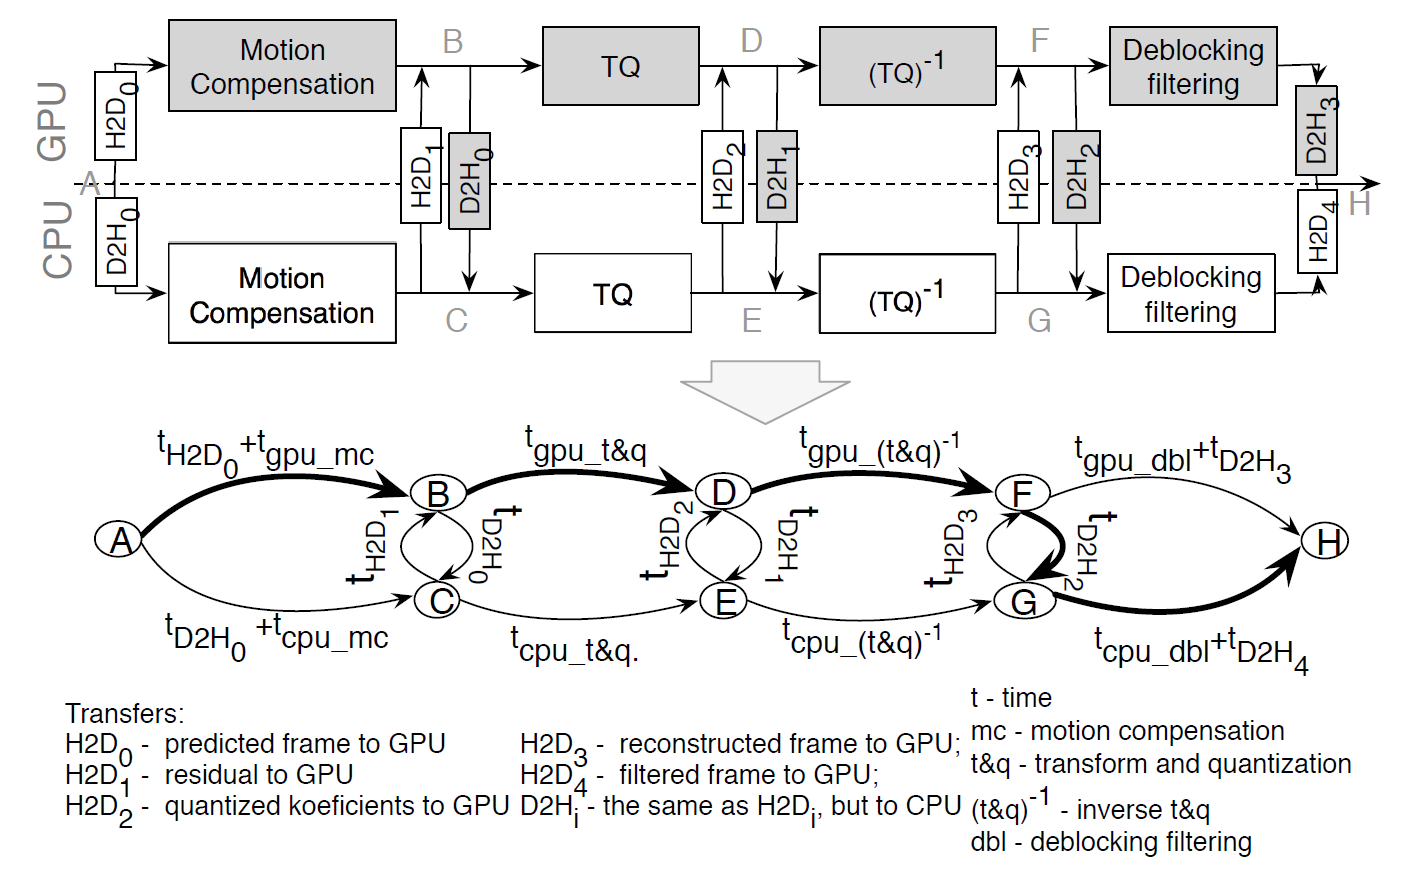
\includegraphics[scale=0.4]{pics/dynamic_model}} % The bounding box is set manually in this example. Useful for some .pdf figures.
\caption{\label{dynamic_model}{\it Construction of weighted DAG from the data-flow diagram of H.264/AVC and
a possible minimal path (represented in bold) (taken from \cite{Paper2})}}
\end{figure*} % [width=5in,bb= 36 253 574 500]

The load distribution model is characterized by its synchronization parts (upper part of figure \ref{dynamic_model}). As mentioned each step will be measured and shared with the other device to evaluate the distribution of tasks for the next frame. By doing so a weighted directed acyclic graph (DAG) will be obtained  (lower part of figure \ref{dynamic_model}). The bold path shows the possible minimal path of the encoding time for the previous frame.\\

\subsection*{CPU plus GPU parallel encoding
Framework for H.265/HEVC}
\label{sec:paper3}
In \cite{Paper3} the authors used the new H.265 codec (unlike in the other two papers) for their approach. In their work they present a CPU plus GPU parallel encoding framework which targets the critical bottlenecks like Variable Block Size Motion Estimation (VBSME) of the encoding algorithm and optimises the data flow between the two devices. The proposed framework is shown in figure \ref{hevc_framework}

\begin{figure*}[ht]
\centerline{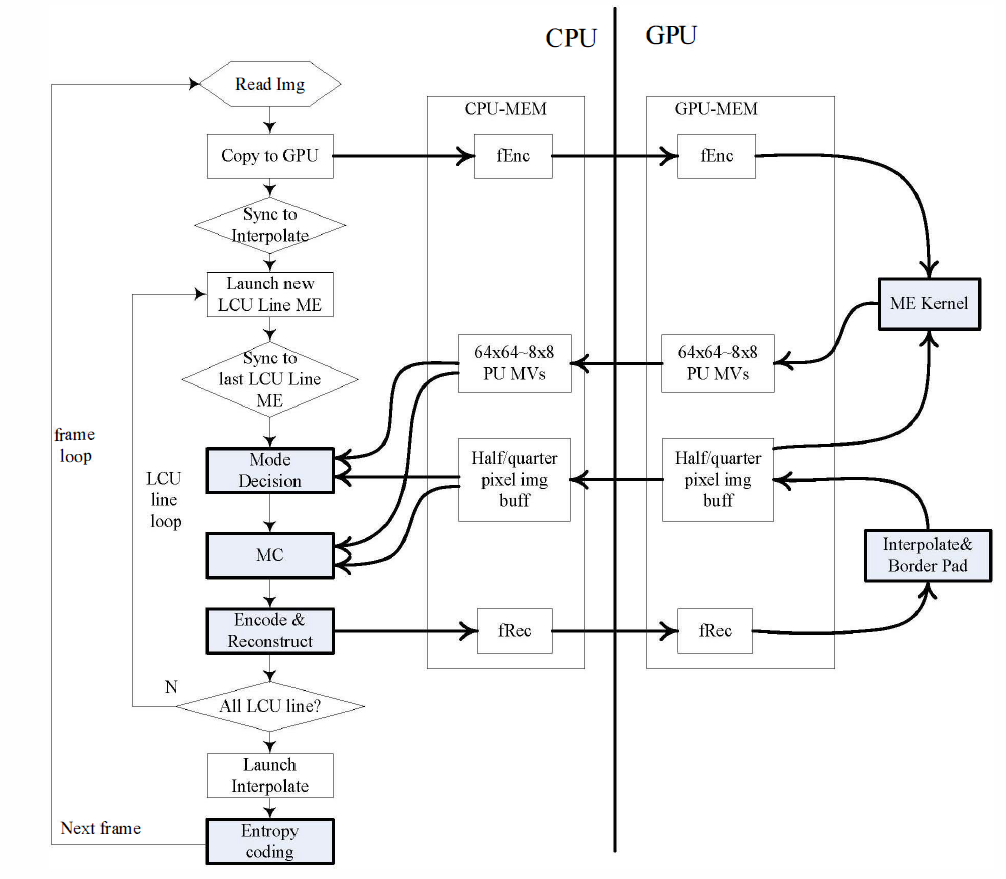
\includegraphics[scale=0.5]{pics/hevc_framework}} % The bounding box is set manually in this example. Useful for some .pdf figures.
\caption{\label{hevc_framework}{\it Parallel encoding framework on CPU plus GPU platform.
The thick lines with arrows represent the dataflow directions. (taken from \cite{Paper3})}}
\end{figure*}

The authors divided the HEVC encoder for their framework into six components: VBSME, mode decision, motion compensation, interpolation, encode plus reconstruction and
entropy coding. The VBSME and Interpolation components,
the right part in figure \ref{hevc_framework}, run on GPU, the others run on
CPU. \\
The ME is like mentioned before very compute intensive and therefore executed on the GPU. In comparison to the other papers the framework considers the MVs dependencies during the ME process. \\
Interpolation is also run on the GPU since it has a fast interpolation unit. The other tasks like mode decision, motion compensation, encode, reconstruct and entropy coding are all run on a CPU.\\
To successfully run the different parts of the algorithm in parallel on both CPU and GPU two synchronisation components are used: 'Sync to Interpolate' and 'Sync to last CTU Line ME'. They ensure that both devices wait for each other if necessary.\\
The mode decision process is according to the authors the bottleneck of this framework and therefore they decided to implement a fast prediction unit partition scheme. This scheme has a maximum of 6 steps and chooses the mode for motion compensation in a faster way than the standard mode decision of the HM encoder \cite{hmencoder}. Of course the speed increase in 
mode decision indicates a possible loss in quality due to some mode decisions that would not be the best.


\section{Experimental Results}
\label{sec:results}
The presented papers all had the goal to research the possibilities to use the parallel performance of the GPU for video encoding. 
\todo{The, typo I suppose should be they} conducted different experiments for speed-up and RD-Performance (quality of the encoded video). 
In this section their experimental set-ups and their results are shown and compared.\\
\\
In the first paper \cite{Paper1} the authors conducted experiments on a PC equipped with one GeForce 8800 GTS PCIe graphics card with 96 stream processors \cite{geforce8800}, 
and an Intel Core 2 Quad Q9400 2.66 GHz CPU with 3.23 GB of RAM. To implement the GPU code, they used NVIDIA's Compute Unified Device Architecture (CUDA) \cite{nvidia2programming}. \\
They conducted multiple experiments with their implemented code on CPU+GPU, where the fast ME was executed on the GPU and compared their results to the JM 14.2 reference software on a single core and on a quad core. 
They used the H.264 high profile with a search range of 64. The chosen tile height was always \textit{L=1}. The video sequences were at HD 720p(1280x720 pixels, 60 frames per second).\\
The result of the quad core comparison is depicted below in figure \ref{tiling_speedup_mc}.
\begin{figure}[H]
\centerline{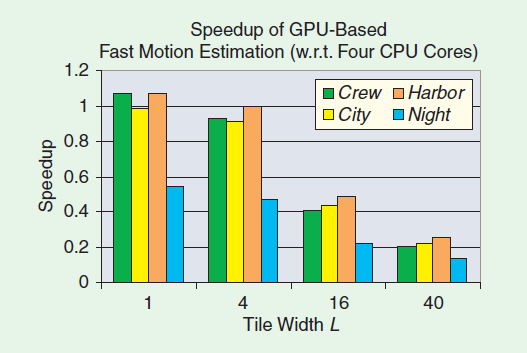
\includegraphics[scale=0.4]{pics/tiling_speedup_mc}} % The bounding box is set manually in this example. Useful for some .pdf figures.
\caption{\label{tiling_speedup_mc}{
\it Trade-off between tile width and speed-up (taken from \cite{Paper1})
%\footref{ftn:speedup} (tile height \textit{K} is
%equal to one) TODO
.
}}
\end{figure} 

The experiments on the speed-up indicate that with their tiling approach they reach a minimal speed-up of around 5\% for certain sequences like \textit{Crew} and \textit{Harbor} at a tile width of \textit{L}=1. 
In every other constellation of tile widths the quad core CPU is equally fast or mostly faster than their implementation.\\

\todo{put following sentences into one paragraph make more sense}
As for the evaluation of the RD performance the results showed the average peak signal-to-noise-ration (PSNR) degradation and the average increase in bit rate using different tile sizes, 
measured by Bjontegaard Delta PSNR (BDPSNR) and Bjontegaard Dekta bit rate (BDBR)\footnote{BDPSNR and BDBR are used frequently in the video standardization community \cite{bjontegaard}} respectively.
The results suggest tiling may lead to average degradation between 0.08 dB to 0.4 dB for these sequences with a tile size of \textit{K}=1, \textit{L}=1.
Their loss in quality is of course due to the loss of information on MVs. \\

A possible explanation for the low speed-up might be the access latency of the memory. 
Their encoder is implemented to store the pixel data needed by the GPU in the off-chip memory which generates high access latencies. 
A possible solution would be to use memory coalescing, which means that all the threads would read from the memory at the same time from one memory bank. 
\todo{no, this is not memory coalescing, thread in warp(a group of threads) access consecutive elements stored in memory, they are not in the same one memory bank}
\todo {Thus the frame data has to be sequential inside the memory, I don't get it}, but it would speed-up the memory access enormously.
\todo {another tip here is that with configuration K=1 L=1, maximum number of threads can be launched for one frame, therefore more parallelism can be exploited}\\

The second paper \cite{Paper2} also used the JM encoder as reference software, but in version 17.2. They ran their experiments on PCs with an Intel Core i/ with 3Ghz and an Intel Core 2 Quad with 2 Ghz. Both Platforms have 4GB memory and use a Geforce GTX 580. The results presented here are regarding the Core 2 Quad, to better compare it with the other papers.\\
The video sequences used were at 1080p (1920x1080) and they chose a search range of 32.\\
Their implementation of the dynamic distribution model was compared to the following:\\
\begin{itemize}
\item \textbf{CPU-only}: the whole encoder is implemented in the CPU
\item \textbf{GPU-only}: the whole encoder is implemented in the GPU
\item \textbf{Chen\_original}: method proposed by Chen \cite{chen2008h}, where the ME, SME and
interpolation modules are statically offloaded to the GPU
(the rest are kept in the CPU)
\item \textbf{Chen\_optimized}: Chen's encoder \cite{chen2008h}, optimized with \\OpenMP and SSE4 vec-
torization techniques
\item  \todo{\textbf{Proposed}: presented dynamic load distribution strategy, why their implementation would compare to the proposed, I think this one should be removed}
\end{itemize}
The author didn't clearly specify the GPU-only implementation and  what it specifically means for the different parts of the algorithm and is therefore ignored in this article.\\
In figure \ref{dynamic_model_result} the results of the experiment is shown.

\begin{figure}[H]
\centerline{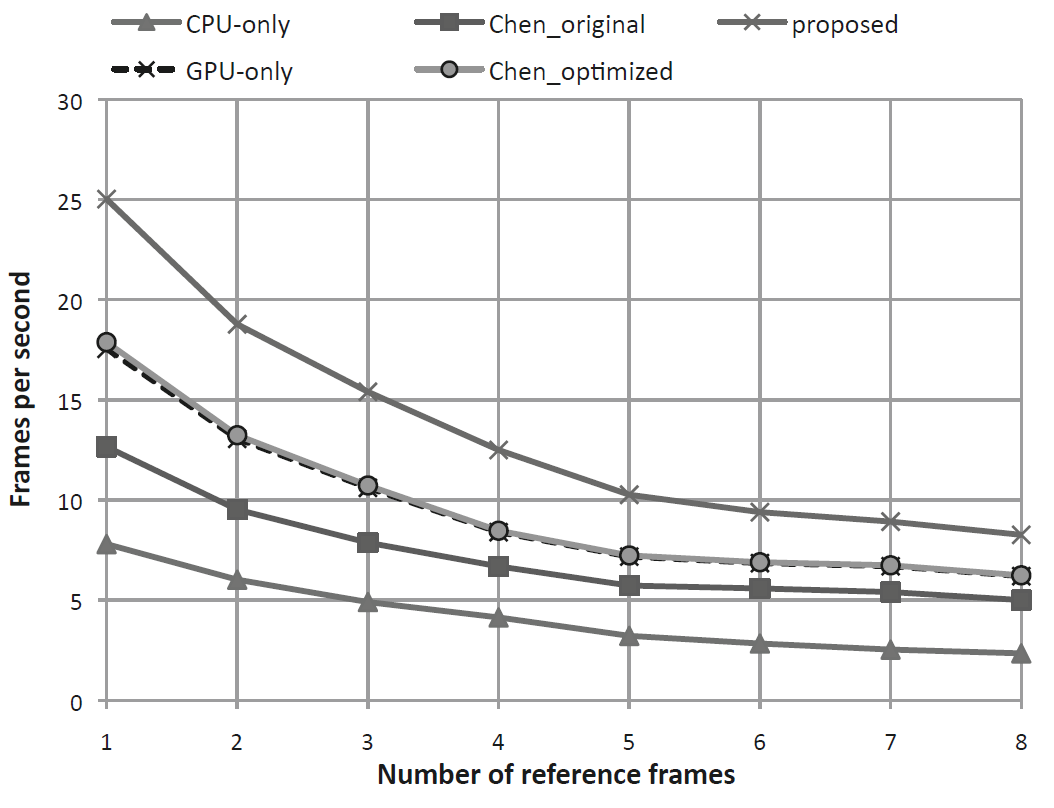
\includegraphics[scale=0.3]{pics/dynamic_model_result}} % The bounding box is set manually in this example. Useful for some .pdf figures.
\caption{\label{dynamic_model_result}{\it Encoded frames per second (fps)
 for a varying number of RFs, using the 1920x1080  video format.
  Comparison of the proposed approach with CPU-only, GPU-only and the
  approach proposed by Chen (taken from \cite{Paper2}).}}
\end{figure}

The proposed method reaches a speed-up of around 25\% compared to the Chen optimized encoder, around 500\% compared to the CPU only, respectively. Besides the increased performance of the proposed dynamic distribution model, the approach of the authors guarantees a certain independence from the adopted devices. In case either the CPU or the GPU is slow, the distribution model would have a different minimal path than with different devices. Of course the proposed method will only guarantee a speed-up if the distribution between the devices is useful. In case only the CPU is fast, there would be an immense overhead for the communication between CPU and GPU without any distribution to the GPU. 
Therefore it has to be taken into consideration, that the dynamic load distribution model is only of good use in specific cases of hardware configuration.\\
\\ 
The third paper \cite{Paper3} used the workstation Z620 from Hewlett-Packard with a NVIDIA Tesla C2050 GPU (448 CUDA cores at a clock rate of 1.15Ghz) for their experiments. The used CPU is not mentioned in the article.\\
They evaluated the acceleration performance of the improved VBSME on GPU and the RD in comparison to the reference encoder (HM9.0 \cite{hmencoder}). The proposed framework runs on CPU and GPU, \todo{typo seriell} and parallel. 
The reference encoder is only executed on a single CPU core. The search range is 64x64 with the full search strategy. They used two test video sequences with different
resolutions: \textit{BasketballDrive} (1920x1080 - 50fps) and
\textit{Traffic} (2560x1600 - crop).\\
Th results of their experiments regarding the speed-up are shown in table \ref{hevc_table_result}

\begin{table*}[ht]
  \centering
  \begin{tabular}{cccc}
    \textbf{Sequence} & \textbf{CPU(fps)} & \textbf{GPU(fps)} & \textbf{Speedup ratio in \%} \\
    Traffic\_2560x1600 & 0.21 & 23.77 & 113.2\\
    ParkScreen\_1920x1080 & 0.69 & 77.76 & 112.7\\
 \end{tabular}
 \caption{ \label{hevc_table_result}{\it Speedup gains on different video sequences (data taken from \cite{Paper3})}}
\end{table*}

The proposed CPU + GPU framework reached an immense speed-up of about 113 times the speed of the encoding time of the single core with the HM9.0 encoder. The authors reached an impressive result in their experiments but didn't quite take a width use of their setup into account. Full search is usually not used for ME because then the whole reference frame is scanned and therefore it takes a lot of time. They also compared their optimized results to the HM9.0 encoder which was executed on a single thread on a CPU not specified in the paper. The authors don't go into detail about any further optimizations for their framework or for the HM encoder and therefore it is possible that in a slightly different setup the speed-up would not be as big as in the experiments. \\
Another experiment they conducted was regarding the quality of the encoded video. Due to the fast decision mode they implemented they predicted some quality loss. In figure \ref{hevc_rd_result} the results are presented.\\

\begin{figure}[H]
\centerline{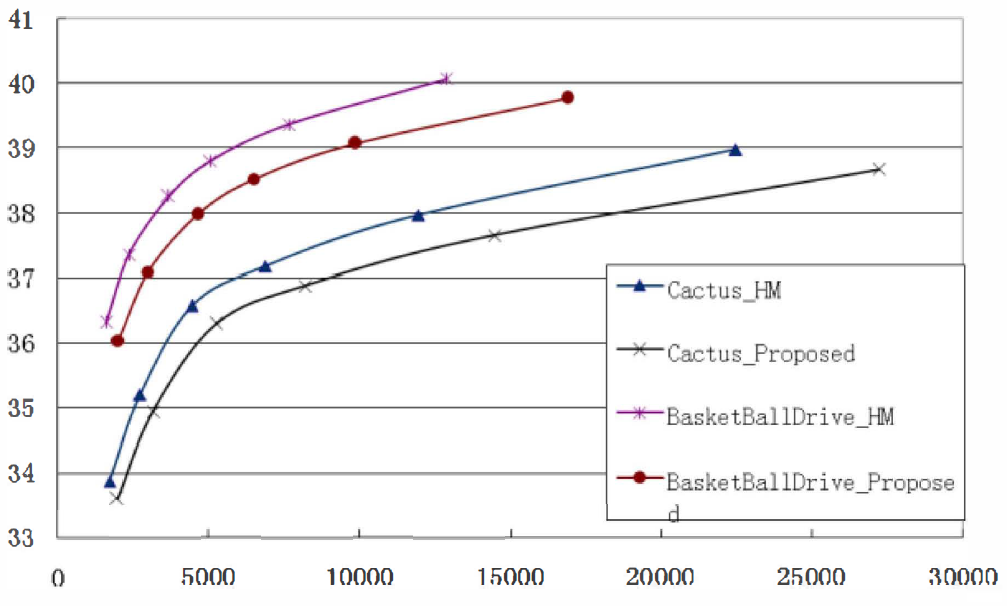
\includegraphics[scale=0.3]{pics/hevc_rd_result}} % The bounding box is set manually in this example. Useful for some .pdf figures.

\caption{\label{hevc_rd_result}{\it RD curve of the HM encoder and the proposed encoder. (taken from \cite{Paper3}}}
\end{figure}

The diagram shows the RD curves of the two encoders. From these RD curves, it can be seen that the RD performance degradation of the proposed
encoder with fast CU partition decision algorithm is about
0.7 dB degradation (calculated by BDPSNR \cite{bjontegaard}), which is a significant loss in quality.
\todo{you can criticize more, not only the DB, but also mention the degradation of bit rate, their solution increases 40\% more bit rate, which should be avoided.}\\
\\
The three papers all presented results regarding the use of the parallel performance of the GPU for certain tasks of the H.264 or H.265 codec.
Paper 1 is the only one that is using a fast ME algorithm\todo{are you sure the second paper also use full search? please check} and therefore no full search for their experiments. 
Full search is for real applications usually not an option and therefore not the best comparable setup.\\
Despite that the first paper didn't really reach a mentionable speed-up with even a great loss of quality. 
The experiments of the third paper show a similar result towards the quality (even worse) due to the fast decision mode. 
But in comparison to the first paper they reached a high speed-up, although the experimental setup is not enough specified. 
The second paper seems to be the most legit regarding the experimental setup and results. They compared they model to an optimized algorithm and specified the machines it was tested on. 
They also used \todo{are you sure the second paper also use full search? please check} a full search algorithm and reached a speed-up between 1.5 - 2 times which seems way more legit then the 113 times from the third paper. 

\section{Conclusion}
\label{sec:conclusion}
This paper reviewed three different approaches to utilize parallel power of modern computers for the means of reaching a better video encoding performance using either the previous (H.264/AVC) or the current (H.265/HEVC) standard video codec. \\
In particularly the first paper \cite{Paper1} proposed a GPU based fast motion estimation framework for H.264/AVC with the main idea of tiling a frame. The ME of each tile is then to be calculated on a different GPU thread to reach a high level of parallelization. For this approach was only a case study, the results only indicated, that it is possible to reach a high level of parallelization, but with the implemented framework didn't prove to be efficient in speed or quality.\\
The second work \cite{Paper2} proposed a dynamic model for parallel H.264/AVC video encoding on hybrid GPU+CPU. Their main idea was to evaluate at runtime which device is more suitable for different tasks of the encoding algorithm. The implemented framework used the dynamic model and distributed every task according to the runtime analysis. Given the experimental results and the speed-ups they reached this dynamic model showed a lot of potential for certain hardware set-ups.\\
The last paper \cite{Paper3} used in contrary to the other two articles the H.265/HEVC codec. It described a proposal for a parallel CPU+GPU framework, that aims to execute VBSME and Interpolation on the GPU while executing every other task of the encoding algorithm on the CPU. Two synchronisation units take care of the communication between the devices and the steps they execute. A fast decision mode algorithm was introduced to approach the problem of the decision mode being the bottleneck of the framework. The results indicated a certain quality loss, but showed a huge speed-up.\\
\\
Despite the first reviewed paper the other two showed potential improvements for the encoders of the used video codecs. Due to their limitations towards specific hardware like in the second paper or the rather poor comparison of results in the third paper. \\
All three papers used high performance graphic cards for their experiments but none took the possibility of a multi-chip GPU or an multi-GPU system like SLI vom NVIDIA or Crossfire from AMD into account. \cite{multigpu} for instance created a job system to do just that. Combining the possible parallelization of certain algorithm of the video encoding process with the possible distribution to multiple GPUs would properly decrease the encoding time even more. But of course new challenges regarding data dependency would arise. Future work in that field are only targeting the current codec H.265. Since it has been released different papers have already been released on improving the parallel capability of it, although the codec already includes parallel structures like tiles and wavefront parallel processing.

%------------------------------------------------



%\section{Methods}
%
%Maecenas sed ultricies felis. Sed imperdiet dictum arcu a egestas.
%\begin{compactitem} 
%
%\item Donec dolor arcu, rutrum id molestie in, viverra sed diam 
%
%\item Curabitur feugiat 
%
%\item turpis sed auctor facilisis 
%
%\item arcu eros accumsan lorem, at posuere mi diam sit amet tortor 
%
%\item Fusce fermentum, mi sit amet euismod rutrum 
%
%\item sem lorem molestie diam, iaculis aliquet sapien tortor non
%nisi 
%
%\item Pellentesque bibendum pretium aliquet \end{compactitem} \lipsum{[}4{]}
%% Dummy text
%
%
%%------------------------------------------------
%
%
%
%\section{Results}
%
%\begin{table}[H]
%\caption{Example table}
%
%
%\centering %
%\begin{tabular}{llr}
%\toprule 
%\multicolumn{2}{c}{Name} & \tabularnewline
%\cmidrule(r){1-2} First name  & Last Name  & Grade \tabularnewline
%\midrule 
%John  & Doe  & $7.5$ \tabularnewline
%Richard  & Miles  & $2$ \tabularnewline
%\bottomrule
%\end{tabular}
%\end{table}
%
%
%\lipsum{[}5{]} % Dummy text
%
%
%\begin{equation}
%e=mc^{2}\label{eq:emc}
%\end{equation}
%
%
%\lipsum{[}6{]} % Dummy text
%
%
%%------------------------------------------------
%
%
%
%\section{Discussion}
%
%
%\subsection{Subsection One}
%
%\lipsum{[}7{]} % Dummy text
%
%
%
%\subsection{Subsection Two}
%
%\lipsum{[}8{]} % Dummy text


%----------------------------------------------------------------------------------------
%	REFERENCE LIST
%----------------------------------------------------------------------------------------



%\section{References}
\newpage

\bibliographystyle{ieeetran}
%\bibliographystyle{apalike}	% (uses file "plain.bst")
\bibliography{bib}		% expects file "literatur.bib"


%----------------------------------------------------------------------------------------


\end{multicols}
\end{document}